\documentclass[english,reprint, aps, prl,superscriptaddress, showpacs,
showkeys, longbibliography, amsmath, amssymb, floatfix]{revtex4-1} 
\pdfoutput=1

\usepackage{fullpage}
\usepackage{cmap}
\usepackage[T1,T2A]{fontenc}
\usepackage[utf8]{inputenc}
\usepackage[french,main=english]{babel}
\usepackage{amsthm}
\usepackage{mathrsfs}
\usepackage{bbold}
\usepackage{wesa}
\usepackage{graphicx}
\usepackage{verbatim}
\usepackage[backref=false]{hyperref}
\usepackage{booktabs}
\usepackage{multirow}
\usepackage[braket,qm]{qcircuit}
\usepackage{color}
\usepackage[usenames,dvipsnames]{xcolor}
\usepackage{framed}
\usepackage{comment}
\usepackage{xparse}

\theoremstyle{plain}
\newtheorem{thm}{Theorem}
\newtheorem{lemma}{Lemma}[thm]
\newtheorem{cor}{Corollary}[thm]
\newtheorem{assumption}{Assumption}
\newtheorem{fact}{Fact}
\theoremstyle{definition}
\newtheorem{definition}{Definition}
\newtheorem{condition}[assumption]{Condition}
\setcounter{thm}{2}

\DeclareUnicodeCharacter{0229}{\c{e}}

\newcommand{\Hilb}{\mathcal{H}}
\newcommand{\events}{\ensuremath{\mathcal{E}}}
\newcommand{\qevents}{\ensuremath{\mathcal{E}}}
\newcommand{\pmeas}{\ensuremath{\mu}}
\newcommand{\imposs}{\ensuremath{\left[0,0\right]}}
\newcommand{\likely}{\ensuremath{\left[\tfrac{1}{2},1\right]}}
\newcommand{\unlikely}{\ensuremath{\left[0,\tfrac{1}{2}\right]}}
\newcommand{\necess}{\ensuremath{\left[1,1\right]}}
\newcommand{\unknown}{\ensuremath{\left[0,1\right]}}
\newcommand{\midd}{\ensuremath{\left[\tfrac{1}{4},\tfrac{3}{4}\right]}}
\newcommand{\fket}[1]{{|#1\rangle}}
\newcommand{\fproj}[1]{|#1\rangle\langle #1|}
\newcommand{\proj}[1]{\op{#1}{#1}}
\newcommand{\ps}{\texttt{+}}
\newcommand{\ms}{\texttt{-}}
\newcommand{\set}[2]{\ensuremath{\left\{ {#1}\mathrel{}\middle|\mathrel{}{#2}\right\} }}
\newcommand{\Tr}{\ensuremath{\mathop{\mathrm{Tr}}\nolimits}}
\allowdisplaybreaks
\newcommand{\coreBorn}{\ensuremath{\overline{\Hilb}}}
\newcommand{\mul}[1][]{\ensuremath{\mu^{L{#1}}}}
\newcommand{\mur}[1][]{\ensuremath{\mu^{R{#1}}}}
\setcounter{secnumdepth}{3}
\newcommand{\rmd}{d}
\newcommand{\rmi}{i}
\lineskiplimit=1pt
\newcommand{\ultramodular}{\mathcal{M}}
\newcommand{\ultramodularL}[1][]{\ensuremath{\ultramodular^{L{#1}}}}
\newcommand{\ultramodularR}[1][]{\ensuremath{\ultramodular^{R{#1}}}}
\newcommand{\muB}{\ensuremath{\mu^{B}}}
\newcommand{\eventsC}{\ensuremath{\events_{C}}}

\newcommand{\says}[3]{\begin{framed}\begin{minipage}{0.9\linewidth}\color{#1}{#2 says: #3}\end{minipage}\end{framed}}
\newcommand{\amr}[1]{\says{green}{Amr}{#1}}
\newcommand{\yutsung}[1]{\says{purple}{Yu-Tsung}{#1}}
\newcommand{\gerardo}[1]{\says{OliveGreen}{Gerardo}{#1}}
\newcommand{\andy}[1]{\says{blue}{Andy}{#1}}
% \excludecomment{suggest}
\NewDocumentEnvironment{suggest}{m m O{}}{#1{TEXT \##2 would go here. #3}}{#1{TEXT \##2 end here.}}

\newcommand{\happen}{\text{H}}
\newcommand{\notHappen}{\text{N}}
\newcommand{\missing}{?}

\begin{document}

\title{Response to the Referee Report for \texorpdfstring{\\}{}
``Quantum Interval-Valued Probability: Contextuality and the Born Rule''}
\date{\today}

\maketitle

%%%%%%%%%%%%%%%%%%%%%%%%%%%%%%%%%%%%%%%%%%%%%%%%%%%%%%%%%%%%%%%%%%%

\noindent In our QIVPM framework, the Kochen-Specker (KS) theorem is
equivalent to stating that there does not exist a
($\delta$=)$0$-deterministic QIVPM. We further claim
(Thm.~\ref{cor:Kochen-Specker-IVPM}) that there cannot exist any
$\delta$-deterministic QIVPM for $\delta<\frac{1}{3}$ and that there
exist QIVPMs for every $\delta\ge\frac{1}{3}$.  The referee questions
the correctness of Thm.~\ref{cor:Kochen-Specker-IVPM} and the physical
interpretation of $\delta$-determinism. In answer to the question of
correctness, we include below, for the referee's convenience, an
expanded proof. In the remainder of the response, we explain the
physical interpretation of $\delta$-determinism and provide examples
that illustrate why $\frac{1}{3}$ is special.

\subsection*{Expanded Proof of Thm.~3}

We begin with a lemma related $\delta$-deterministic QIVPMs and
0-deterministic QIVPMs. 

\begin{lemma} 
  From any $\delta$-deterministic
  QIVPM~$\bar{\mu}:\events\rightarrow\mathscr{I}$ with
  $\delta < \frac{1}{3}$, we can construct the $0$-deterministic QIVPM
  $\bar{\mu}^{\textrm{D}}:\events\rightarrow\left\{
    \imposs,\necess\right\}$ defined as follows:
\begin{equation}
\bar{\mu}^{\textrm{D}}\left(P\right)=\begin{cases}
\imposs\,, & \textrm{ if }\bar{\mu}\left(P\right)\subseteq\left[0,\delta\right]\:;\\
\necess\,, & \textrm{ if }\bar{\mu}\left(P\right)\subseteq\left[1-\delta,1\right]\:.
\end{cases}
\end{equation}
\end{lemma}
The most important part of the proof is to verify the convexity
condition for $\bar{\mu}^{\textrm{D}}$. Because
$\bar{\mu}^{\textrm{D}}$ is 0-deterministic, it is sufficient to
verify the following equation for orthogonal projectors $P_{0}$
and~$P_{1}$,
\begin{equation}
\bar{\mu}^{\textrm{D}}\left(P_{0}+P_{1}\right)=\bar{\mu}^{\textrm{D}}\left(P_{0}\right)+\bar{\mu}^{\textrm{D}}\left(P_{1}\right)\,. \label{eq:QuantumInterval-valuedProbability-Equal}
\end{equation}

When one of $\bar{\mu}^{\textrm{D}}\left(P_{0}\right)$ and $\bar{\mu}^{\textrm{D}}\left(P_{1}\right)$
is $\necess$, say $\bar{\mu}^{\textrm{D}}\left(P_{0}\right)=\imposs$
and $\bar{\mu}^{\textrm{D}}\left(P_{1}\right)=\necess$, we have $\bar{\mu}\left(P_{0}\right)\subseteq\left[0,\delta\right]$
and $\bar{\mu}\left(P_{1}\right)\subseteq\left[1-\delta,1\right]$ which
implies $\bar{\mu}\left(P_{0}+P_{1}\right)\subseteq\left[1-\delta,1+\delta\right]$.
Since $\bar{\mu}\left(P_{0}+P_{1}\right)$ is a subset of $\left[0,1\right]$,
$\bar{\mu}\left(P_{0}+P_{1}\right)$ must be a subset of $\left[1-\delta,1\right]$,
which implies $\bar{\mu}^{\textrm{D}}\left(P_{0}+P_{1}\right)$ is also
$\necess$ satisfying Eq.~\ref{eq:QuantumInterval-valuedProbability-Equal}.

When both
$\bar{\mu}^{\textrm{D}}\left(P_{0}\right)=\bar{\mu}^{\textrm{D}}\left(P_{1}\right)$
are $\imposs$, we have both $\bar{\mu}\left(P_{0}\right)$ and
$\bar{\mu}\left(P_{1}\right)\subseteq\left[0,\delta\right]$ which
implies
$\bar{\mu}\left(P_{0}+P_{1}\right)\subseteq\left[0,2\delta\right]$.
Since we assume $\delta<\frac{1}{3}$, $\left[0,2\delta\right]$ and
$\left[1-\delta,1\right]$ are disjoint, which implies
$\bar{\mu}\left(P_{0}+P_{1}\right)$ and $\left[1-\delta,1\right]$ are
disjoint. Together with the fact that
$\bar{\mu}\left(P_{0}+P_{1}\right)$ is a subset of either
$\left[0,\delta\right]$ or $\left[1-\delta,1\right]$,
$\bar{\mu}\left(P_{0}+P_{1}\right)$ must be a subset of
$\left[0,\delta\right]$, which implies
$\bar{\mu}^{\textrm{D}}\left(P_{0}+P_{1}\right)=\imposs$ and hence
also satisfying Eq.~\ref{eq:QuantumInterval-valuedProbability-Equal}.

\begin{thm}[Finite-precision Extension of the Kochen-Specker Theorem]
\label{cor:Kochen-Specker-IVPM} Given a Hilbert space $\Hilb$ of 
dimension~$d\ge3$, there is no $\delta$-deterministic QIVPM for 
$\delta<\frac{1}{3}$.\end{thm}
The proof is by contradiction: Suppose there is a $\delta$-deterministic 
QIVPM~$\bar{\mu}:\events\rightarrow\mathscr{I}$. By the previous
lemma, we can construct a 0-deterministic QIVPM but by Thm.~2 in the
paper, such 0-deterministic QIVPMs do not exist. 

\subsection*{Experimental Data and \texorpdfstring{$\delta$}{delta}-determinism} 

To the best of our understanding, the argument against
$\delta$-determinism by the referee assumes that the parameter
$\delta$ is \emph{exclusively} related to the density of states
defined in a general Hilbert space. This is indeed Meyer's great
insight and the main assumption in his proof that using the field of
rationals nullifies the KS theorem.  In other words, Meyer attributes
finite-precision errors to the description of the states.

In addition to responses like Mermin's that argue against Meyer's
interpretation but accept his framework, there have been responses
that argue that the effect of finite-precision measurements on the KS
theorem requires a different approach altogether (see for example Ax
and Kochen as cited by Cabello 2002). Our approach is agnostic about
attributing elements of reality to the state function (as Meyer
did). We simply attribute lack of certainty to the measured results
through the use of an instrument. Thus, the parameter $\delta$ in our
framework reflects insufficient knowledge of the experimenter, which
could be due to a variety of reasons related to imperfections of
devices. For example, a typical question that an experimenter may not
be able to answer accurately would be ``did an electron land in the
left half or the right half of the screen''? There are cases in which
the electron would land too close to the middle of the screen for the
experimenter to be able to determine with certainty that it was left
or right of the center. We simply record this imprecision in the
probability we assign to events, and use the axioms of probability
theory to argue that a sharp transition occurs when the imprecision
reaches a certain value.

In an experimental setup, $\delta$ is calculated as follows. To
determine the probability of any event, we typically repeat an
experiment $n$ times and count the number of times we witness the
event. This assumes that for each run of the experiment we can
determine, using our apparatus, whether the event occurred or
not. Assume an event has an ideal mathematical probability of $0$, and
we repeat the experiment $100$ times. In a perfect world we should be
able to refute the event $100$ times and calculate that the
probability is $0$. We might also observe the event $2$ times and
refute it $98$ times and therefore calculate the probability to be
$0.02$. Note that this situation assumes perfect measurement
conditions and remains within the context of conventional
(real-valued) probability theory. The question we focus on is what
happens if we are only able to refute it $97$ times and are
\emph{uncertain} $3$ times? This is quite common in actual
experiments. Mathematically we can model this idea by stating that the
probability of the event is in the range $\left[0,0.03\right]$ which
says that the probability of the event could be $0$, $0.01$, $0.02$,
or $0.03$ as each the three missing records could either be evidence
for the event or against it. We just cannot nail it down given the
current experimental results and therefore represent them as a
($\delta=$)$0.03$-deterministic probability measure. The interesting
observation is that the axioms of probability theory (like additivity
and convexity) impose enough constraints on the structure of
interval-valued quantum probability measures to make them robust in
the face of small $\delta$'s.

To see this idea in the context of a quantum experiment, consider
a three-dimensional Hilbert space and an experiment repeated $12$
times. By the KS theorem, it is impossible to build a probability
measure that maps every projection to either $0=\frac{0}{12}$ or
$1=\frac{12}{12}$. That is, the following assignment~$\bar{\mu}_{0}$
is not a QIVPM
\begin{center}
\begin{tabular}{cc}
\toprule 
\addlinespace
$P$  & $\bar{\mu}_{0}\left(P\right)$\tabularnewline
\midrule
\midrule 
\addlinespace
$\mathbb{0}$  & $\imposs$\tabularnewline
\midrule 
\addlinespace
All one-dimensional projectors  & $\left[0,0\right]$\tabularnewline
\midrule 
\addlinespace
All two-dimensional projectors  & $\left[1,1\right]$\tabularnewline
\midrule 
\addlinespace
$\mathbb{1}$  & $\necess$\tabularnewline
\bottomrule
\end{tabular}
\par\end{center}

Now consider what happens if $\frac{1}{4}$ of the data for every
one-dimensional projector is missing. A potential account of this
degradation is to assign to each event $P$ the entire range of possibilities
$\bar{\mu}_{1}(P)$: 
\begin{center}
\begin{tabular}{cc}
\toprule 
\addlinespace
$P$  & $\bar{\mu}_{1}\left(P\right)$\tabularnewline
\midrule
\midrule 
\addlinespace
$\mathbb{0}$  & $\imposs$\tabularnewline
\midrule 
\addlinespace
All one-dimensional projectors  & $\left[0,\tfrac{1}{4}\right]$\tabularnewline
\midrule 
\addlinespace
All two-dimensional projectors  & $\left[\tfrac{3}{4},1\right]$\tabularnewline
\midrule 
\addlinespace
$\mathbb{1}$  & $\necess$\tabularnewline
\bottomrule
\end{tabular}
\par\end{center}

\noindent This measure is not a valid QIVPM because it does not satisfy
the convexity condition: for any two orthogonal one-dimensional events
$P_{0}$ and $P_{1}$, the convexity condition requires $\bar{\mu}_{1}\left(P_{0}+P_{1}\right)\subseteq\bar{\mu}_{1}\left(P_{0}\right)+\bar{\mu}_{1}\left(P_{1}\right)$,
but $\bar{\mu}_{1}\left(P_{0}+P_{1}\right)=\left[\tfrac{3}{4},1\right]$
which is not a subset of $\left[0,\tfrac{1}{2}\right]=\bar{\mu}_{1}\left(P_{0}\right)+\bar{\mu}_{1}\left(P_{1}\right)$.
Interestingly, it is impossible to find any probability measure that
would be consistent with these observations as the interval $\left[\tfrac{3}{4},1\right]$
is completely disjoint from the interval $\left[0,\tfrac{1}{2}\right]$
and no amount of shifting of assumptions regarding the precise outcome
of the missing observations could change that disjointness. However,
a sharp transition occurs when $\delta=\tfrac{1}{3}$ as shown next.

In case the missing data reaches $\frac{1}{3}$, the probability measure
that assigns to each event the entire range of possibilities is: 
\begin{center}
\begin{tabular}{cc}
\toprule 
\addlinespace
$P$  & $\bar{\mu}_{2}\left(P\right)$\tabularnewline
\midrule
\midrule 
\addlinespace
$\mathbb{0}$  & $\imposs$\tabularnewline
\midrule 
\addlinespace
All one-dimensional projectors  & $\left[0,\tfrac{1}{3}\right]$\tabularnewline
\midrule 
\addlinespace
All two-dimensional projectors  & $\left[\tfrac{2}{3},1\right]$\tabularnewline
\midrule 
\addlinespace
$\mathbb{1}$  & $\necess$\tabularnewline
\bottomrule
\end{tabular}
\par\end{center}

\noindent This is also not a valid probability measure by the same
argument as above. However, in this case $\bar{\mu}_{2}\left(P_{0}+P_{1}\right)=\left[\tfrac{2}{3},1\right]$
and $\left[0,\tfrac{2}{3}\right]=\bar{\mu}_{2}\left(P_{0}\right)+\bar{\mu}_{2}\left(P_{1}\right)$
have a common point. And hence by assuming that the missing data for
one-dimensional projectors always support the associated event, while
those for two-dimensional projectors always refute the event, we can
find the following probability measure which can verified to be a
valid QIVPM and which is consistent with the experimental data: 
\begin{center}
\begin{tabular}{cc}
\toprule 
\addlinespace
$P$  & $\bar{\mu}_{2}'\left(P\right)$\tabularnewline
\midrule
\midrule 
\addlinespace
$\mathbb{0}$  & $\imposs$\tabularnewline
\midrule 
\addlinespace
All one-dimensional projectors  & $\left[\tfrac{1}{3},\tfrac{1}{3}\right]$\tabularnewline
\midrule 
\addlinespace
All two-dimensional projectors  & $\left[\tfrac{2}{3},\tfrac{2}{3}\right]$\tabularnewline
\midrule 
\addlinespace
$\mathbb{1}$  & $\necess$\tabularnewline
\bottomrule
\end{tabular}
\par\end{center}

A similar situation happens when more than $\frac{1}{3}$ of data
is missing. In particular, having half of the data missing, the probability
measure that assigns to each event the entire range of possibilities
is already a QIVPM:
\begin{center}
\begin{tabular}{cc}
\toprule 
\addlinespace
$P$  & $\bar{\mu}_{3}\left(P\right)$\tabularnewline
\midrule
\midrule 
\addlinespace
$\mathbb{0}$  & $\imposs$\tabularnewline
\midrule 
\addlinespace
All one-dimensional projectors  & $\left[0,\tfrac{1}{2}\right]$\tabularnewline
\midrule 
\addlinespace
All two-dimensional projectors  & $\left[\tfrac{1}{2},1\right]$\tabularnewline
\midrule 
\addlinespace
$\mathbb{1}$  & $\necess$\tabularnewline
\bottomrule
\end{tabular}
\par\end{center}

The above arguments could be summarized and illustrated using the
following figure: 
\begin{center}
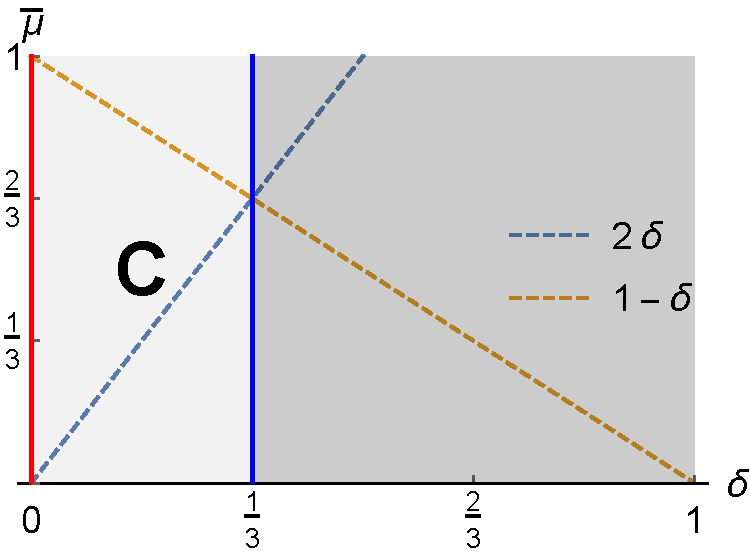
\includegraphics[scale=0.5]{prop_letter_ajhs_referee_response_nb} 
\par\end{center}

\noindent The region to the left of the vertical line at
$\delta=\frac{1}{3}$ is where we assume small measurement degradation;
in that region our extension of the KS theorem definitely demonstrates
contextuality ({\bf{\sf C}}). In the region to the right, the degradation of the data
is large and our extension of the KS theorem no longer refutes other
explanations for the experimental data.


\end{document}


\subsection*{Mermin-Peres ``Magic Square''}

We are going to phrase our results in a different way. Since $\bar{\mu}_{0}$
maps every projectors to $\imposs$ or $\necess$, $\bar{\mu}_{0}$
can predict experimental results deterministically, i.e., it is a
deterministic hidden variable theory despite the fact that $\bar{\mu}_{0}$
is not consistent with the prediction of quantum mechanics. When we
see a set of experimental data with $\frac{1}{3}$ missing represented
by $\bar{\mu}_{2}$, we could not determine whether the original record
is come from the quantum mechanical $\bar{\mu}_{2}'$ or the deterministic
hidden variable theory~$\bar{\mu}_{0}$. The situation changes when
we miss a little less records, say $\frac{1}{4}$. Since we proved
missing $\frac{1}{4}$ of the measurement results of a hidden variable
theory cannot be consistent with any valid QIVPM, symmetrically missing
$\frac{1}{4}$ of the measurement results of a valid QIVPM cannot
be consistent with any hidden variable theory.

This same idea can be used to analyze the Mermin-Peres ``magic square''
argument experimentally, while this time we start from a possible
quantum mechanical results, and show that it could be consistent with
a deterministic hidden variable theory if missing enough records.
The missing records for the Mermin-Peres ``magic square'' could
be much less than the previous examples, because the Mermin-Peres
``magic square'' does use the full set of observables in a Hilbert
space which imposing less constraints. Consider the nine observables
$\mathbf{O}_{ij}$ with $i$ and $j$ ranging over $\{0,1,2\}$, corresponding
to the Mermin-Peres ``magic square'' used to illustrate the KS theorem:


{\renewcommand{\arraystretch}{2}% 
\begin{center} 
\begin{tabular}{r|@{\quad}c@{\quad}|@{\quad}c@{\quad}|@{\quad}c@{\quad}|} 
$\mathbf{O}_{ij}$~ & $j=0$ & $j=1$ & $j=2$ \\ 
\hline  
$i=0~$ & $\mathbb{1}\otimes\sigma_{z}$  & $\sigma_{z}\otimes\mathbb{1}$  & $\sigma_{z}\otimes\sigma_{z}$ \tabularnewline 
\hline  
$i=1~$ & $\sigma_{x}\otimes\mathbb{1}$  & $\mathbb{1}\otimes\sigma_{x}$  & $\sigma_{x}\otimes\sigma_{x}$ \tabularnewline 
\hline  
$i=2~$ & $\sigma_{x}\otimes\sigma_{z}$  & $\sigma_{z}\otimes\sigma_{x}$  & $\sigma_{y}\otimes\sigma_{y}$ \tabularnewline 
\hline  
\end{tabular}\,.
\par\end{center} 
}

\noindent The observables are constructed using the Pauli matrices
$\left\{ \mathbb{1},\sigma_{x},\sigma_{y},\sigma_{z}\right\} $ whose
eigenvalues are all either~$1$ or $-1$. They are arranged such
that in each row and column, \emph{except the column $j=2$}, every
observable is the product of the other two. In the $j=2$ column,
we have instead that 
\begin{equation}
\mathbf{O}_{02}\mathbf{O}_{12}=-\mathbf{O}_{22}\,.\label{eq:j_2_expectation_value}
\end{equation}

Since the observables in each row and column commute, they can be
measured simultaneously. Assume we measure the observables row-by-row
and then column-by-column, and get the following results, where the
? indicates that we are uncertain about the actual outcome of observables~$\mathbf{O}_{22}$
in the last run:
\begin{center}
\begin{tabular}{l@{\qquad}r@{\qquad}r@{\qquad}r}
\toprule 
\addlinespace
Trials & \multicolumn{3}{c}{Results}\tabularnewline
\midrule
\midrule 
\addlinespace
$0$ & $\mathbf{O}_{00}=-1$ & $\mathbf{O}_{01}=-1$ & $\mathbf{O}_{02}=1$\tabularnewline
\midrule 
\addlinespace
$1$ & $\mathbf{O}_{10}=-1$ & $\mathbf{O}_{11}=-1$ & $\mathbf{O}_{12}=1$\tabularnewline
\midrule 
\addlinespace
$2$ & $\mathbf{O}_{20}=1$ & $\mathbf{O}_{21}=1$ & $\mathbf{O}_{22}=1$\tabularnewline
\midrule 
\addlinespace
$3$ & $\mathbf{O}_{00}=-1$ & $\mathbf{O}_{10}=-1$ & $\mathbf{O}_{20}=1$\tabularnewline
\midrule 
\addlinespace
$4$ & $\mathbf{O}_{01}=-1$ & $\mathbf{O}_{11}=-1$ & $\mathbf{O}_{21}=1$\tabularnewline
\midrule 
\addlinespace
$5$ & $\mathbf{O}_{02}=1$ & $\mathbf{O}_{12}=1$ & $\mathbf{O}_{22}=?$\tabularnewline
\bottomrule
\end{tabular}
\par\end{center}

If the undetermined result $?$ is $-1$, this table is consistent
with Eq.~(\ref{eq:j_2_expectation_value}) and the predictions of
quantum mechanics. If the undetermined result $?$ is $1$, every
observable has a definite measurement result, and form a deterministic
hidden variable theory although they are not completely consistent
with the prediction of quantum mechanics.
